\documentclass[../main.tex]{subfiles}
\graphicspath{{\subfix{../figures/}}}
%
\begin{document}
\section{动态建模}
\subsection{状态图}
%
用餐人员状态:
\begin{itemize}
  \item {登录状态}:用餐人员扫描二维码登录食堂APP。
  \item {点菜状态}:用餐人员选择菜品和份数。
  \item {结算状态}:用餐人员进行结算。
  \item {等待状态}:用餐人员等待取餐。
  \item {取餐状态}:用餐人员到窗口取餐。
  \item {完成状态}
\end{itemize}

\begin{figure}[H]
  \begin{center}
    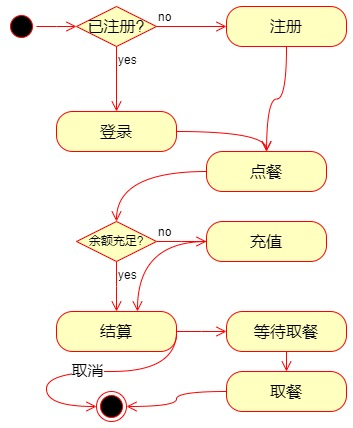
\includegraphics[width=0.45\textwidth]{用餐人员状态图.jpg}
  \end{center}
  \caption{用餐人员状态图}
\end{figure}

工作人员状态:
\begin{itemize}
  \item 等待状态:工作人员等待配餐任务。
  \item 配餐中状态:工作人员正在为用餐人员配餐。
  \item 完成状态:工作人员完成配餐。
\end{itemize}

\begin{figure}[H]
  \begin{center}
    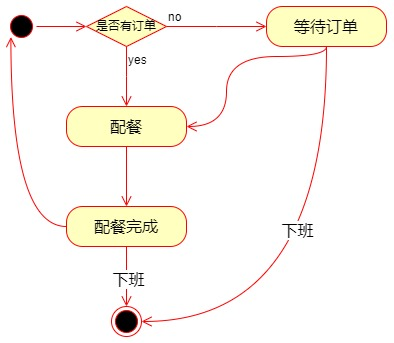
\includegraphics[width=0.45\textwidth]{工作人员状态图.jpg}
  \end{center}
  \caption{工作人员状态图}
\end{figure}

一体机状态:
\begin{itemize}
  \item 待机状态:一体机等待显示配餐任务。
  \item 配餐状态:一体机显示配餐任务列表。
  \item 打印状态:一体机打印餐位号和点餐人员ID的单据。
\end{itemize}

\begin{figure}[H]
  \begin{center}
    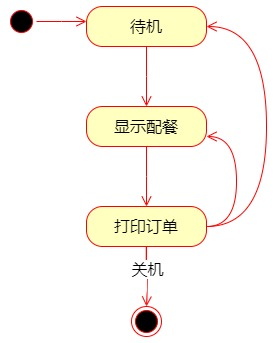
\includegraphics[width=0.45\textwidth]{一体机状态图.jpg}
  \end{center}
  \caption{一体机状态图}
\end{figure}

\subsection{活动图}
\begin{figure}[H]
  \begin{center}
    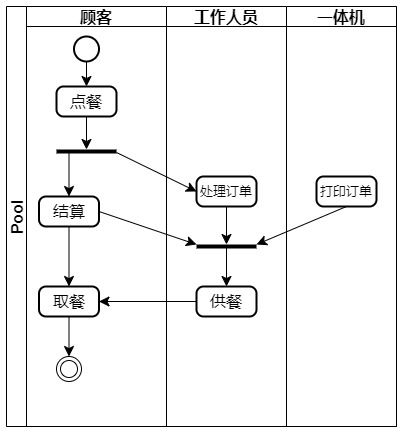
\includegraphics[width=0.65\textwidth]{活动图.jpg}
  \end{center}
  \caption{活动图}
\end{figure}

\subsection{顺序图}
\begin{figure}[H]
  \begin{center}
    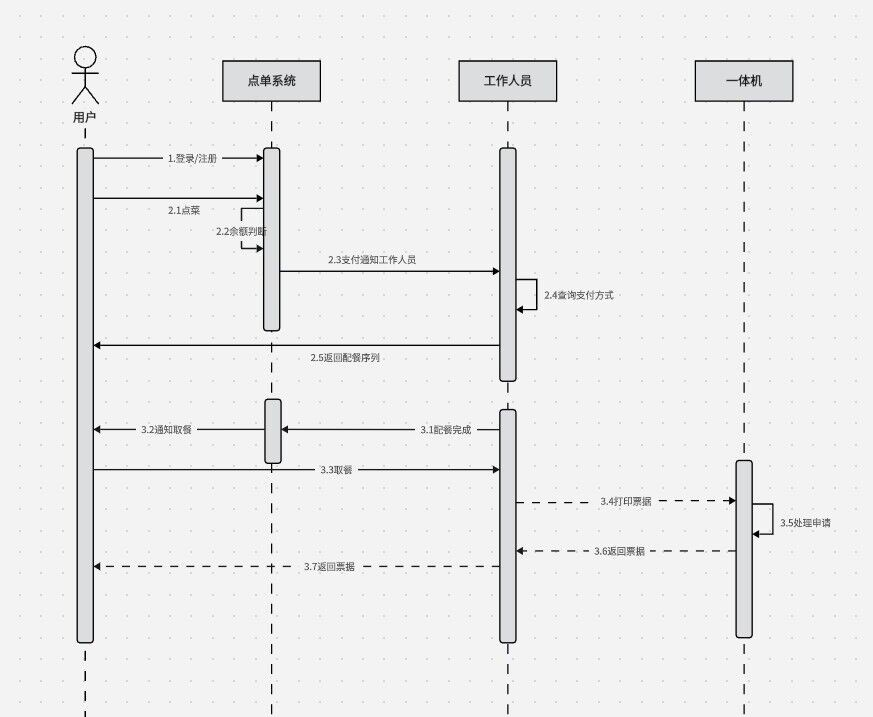
\includegraphics[width=0.65\textwidth]{顺序图.jpg}
  \end{center}
  \caption{顺序图}
\end{figure}

\subsection{合作图}
\begin{figure}[H]
  \begin{center}
    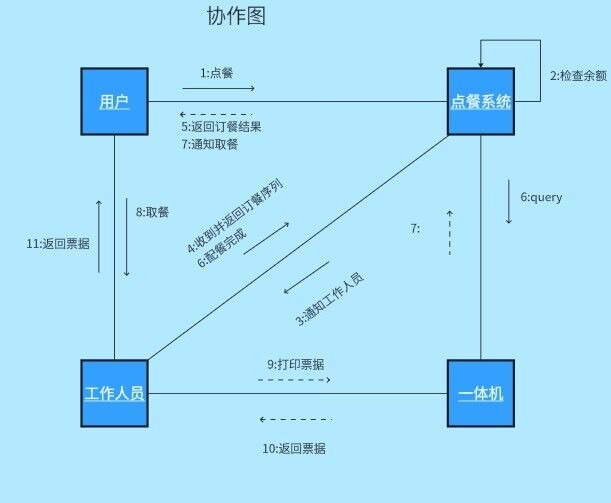
\includegraphics[width=0.65\textwidth]{合作图.jpg}
  \end{center}
  \caption{合作图}
\end{figure}

\end{document}
